%----------------------------------------------------------------------------------------
%    PACKAGES AND THEMES
%----------------------------------------------------------------------------------------
\documentclass[handout, aspectratio=169,xcolor=dvipsnames]{beamer}
\makeatletter
\def\input@path{{theme/}}
\makeatother
\usetheme{CleanEasy}
\usepackage[utf8]{inputenc}
\usepackage{lmodern}
\usepackage[T1]{fontenc}
% \usepackage[brazil]{babel}
\usepackage{fix-cm}
\usepackage{amsmath}
\usepackage{mathtools}
\usepackage{listings}
\usepackage{xcolor}
\usepackage{hyperref}
\usepackage{graphicx} % Allows including images
\usepackage{booktabs} % Allows the use of \toprule, \midrule and \bottomrule in tables
\usepackage{tikz}
\usetikzlibrary{positioning, shapes, arrows, calc, decorations.pathreplacing, arrows.meta, backgrounds, patterns, overlay-beamer-styles}
\usepackage{etoolbox}
\usepackage{animate}
\usepackage{multimedia}
\usepackage{media9}

\usepackage{subfiles}


\newcommand{\bx}{\mathbf{x}}
\newcommand{\by}{\mathbf{y}}
\newcommand{\pd}{p_\text{data}}
\newcommand{\pt}{p_\theta}
\newcommand{\nbx}{\nabla_{\bx}}

\newcommand{\btx}{\mathbf{\tilde{x}}}
\newcommand{\qs}{q_{\sigma}}
\newcommand{\nbtx}{\nabla_{\btx}}

%----------------------------------------------------------------------------------------
%    LAYOUT CONFIGURATION
%----------------------------------------------------------------------------------------
\input{configs/configs}
%----------------------------------------------------------------------------------------

% References from references.bib
\usepackage[backend=bibtex,sorting=none]{biblatex}
\addbibresource{references.bib}


\begin{document}

\section{Week 5 Updates}


\begin{frame}{Old architecture based on LorentzNet}

    $x$ = Cartesian particle 4-momenta, $\phi_\cdot$ = learnable functions, $\psi(\cdot) = \text{sgn}(\cdot) \log(|\cdot| + 1)$, $c = $ hyperparameter, $N = \#$ particles, $|| \cdot ||, \langle \cdot \rangle$ = Minkowski norm and inner product
    \vspace{0.5cm}
    \begin{columns}
        \begin{column}{0.5\textwidth}
            \textbf{LGEB (\cite{gongEfficientLorentzEquivariant2022})}
            \begin{align*}
                m_{ij}^l &= \phi_e(h_i^l, h_j^l, \psi(||x_i^l - x_j^l||), \psi(\langle x_i^l, x_j^l \rangle)) \\
                m_{ij}^l &= \phi_m(m_{ij}^l) \cdot m_{ij}^l
            \end{align*}
            \begin{align*}
                x_i^{l+1} &= x_i^l + \frac{c}{N} \sum\limits_{j \in [N]} \phi_x(m_{ij}^l) \cdot |x_i - x_j|         
            \end{align*}
            \begin{align*}
                h_i^{l+1} &= h_i^l + \phi_h(h_i^l, \sum\limits_{j \in [N]} \phi_w(m_{ij}^l) m_{ij}^l)
            \end{align*}
        \end{column}
        \begin{column}{0.5\textwidth}
            \textbf{Simple LE block}
            \begin{align*}
                m^l_{ij} &= \phi_e(\psi(||x_i^l - x_j^l||), \psi(\langle x_i^l, x_j^l \rangle))\\
                m^l_{ij} &= \phi_m(m^l_{ij}) \cdot m^l_{ij}
            \end{align*}
            \begin{align*}
                x_i^{l+1} &= x_i^l + \frac{c}{N} \sum\limits_{j \in [N]} \phi_x(m_{ij}, g) \cdot |x_j^l - x_i^l|
            \end{align*}
            $g = $ global feature vector (currently time embedding $\phi_t(t)$)
        \end{column}
    \end{columns}
\end{frame}

\begin{frame}{Performance}
    6 layers, 100 epochs, gluons only. 500 generated samples over 32 steps.
    \begin{figure}
        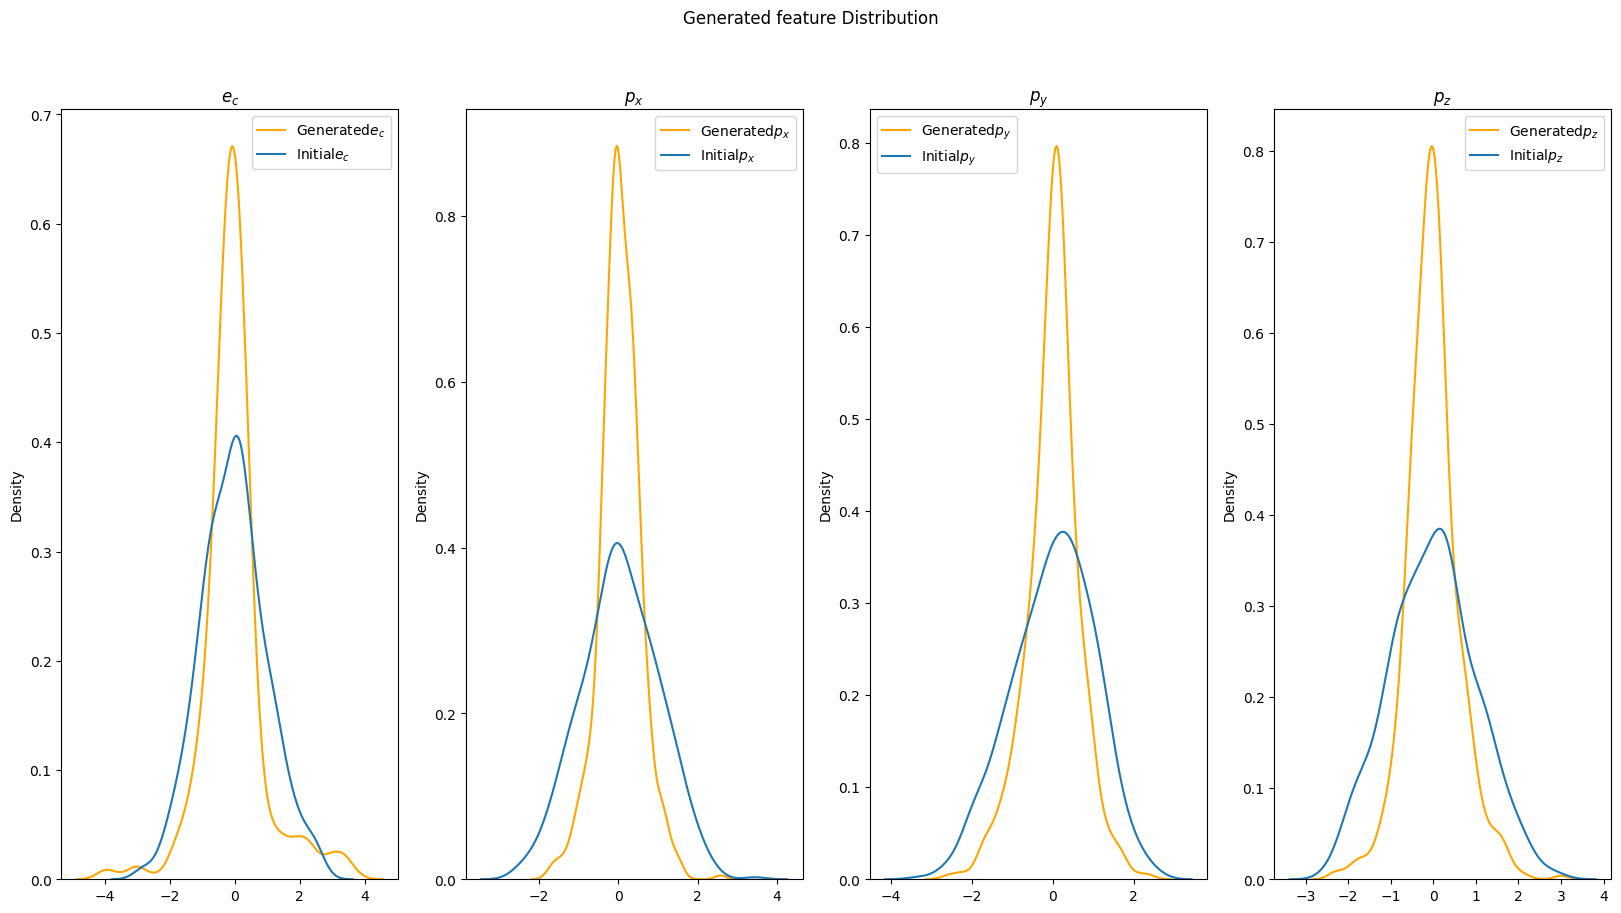
\includegraphics[height=0.6\textheight]{figs/old-model-performance-gluons.png}
    \end{figure}
\end{frame}

\begin{frame}[allowframebreaks]{New architecture}
    \begin{enumerate}
        \item Embed scalar time value to random Fourier features through two fully connected layers with 32 and 64 nodes (following \cite{wuFastPointCloud2023})
        \item Concatenate time embedding with jet conditioning information, which consists of one-hot encoded type, $\eta$, mass, $p_T$, number of constituents
        \item Pass this through a fully connected layer of size 64 to produce the initial global embeddings $g^0$
        \item Concatenate $g^0$ with features $x_1^0 \dots x_N^0$ initialized from the initial distribution $p_0$.
        \item Now, we use $L$ Lorentz-group equivariant layers. \begin{enumerate}
            \item The input to the $l+1$-th layer is $g^l$ and $x^{l}_1 \dots x^l_N$.
            \item Calculate messages $m^l_{ij} = \phi_e^l(\psi(||x_i^l - x_j^l||), \psi(\langle x_i^l, x_j^l \rangle))$
            \item Update the global embedding $$g_{l+1} = \phi^l_{g}(g^0, g^l, \frac{c}{N} \sum\limits_{i, j \in [N]} m^l_{ij} \cdot \phi_m^l(m_{ij}) , \sum\limits_{i, j \in [N]} m^l_{ij} \cdot \phi_m^l(m_{ij}))$$
            \item Feed in the updated global embedding as well as the original embedding to update the graph embeddings $$
            x_i^{l+1} = x_i^{l} + \sum\limits_{j \in N} \phi^l_{x} (g^0, g^{l+1}, m_{ij}) \cdot x_j^l
            $$
            \item Pass the results $g^{l+1}$ and $x_i^{l+1}$ to the next layer
        \end{enumerate}
        \item After the final LE layer, run the particle representations through a final round of message-passing with the final global embedding $$
            x_i^{L+1} = x_i^{L} + \sum\limits_{j \in N} \phi^L_{x} (g^0, g^L, m_{ij}) \cdot x_j^L
        $$
        \item The final output $v_\theta(t, x^0)_i = x_i^L - x_i^0$
    \end{enumerate}
\end{frame}

\begin{frame}{Jet conditioning implementation}
    \begin{itemize}
        \item During training, use the real features corresponding to each jet.
        \item During inference: \begin{itemize}
            \item Use the normalizing flow to generate jet attributes
            \item Round the number of jet constituents and clamp to [4, 150]
            \item Generate masks corresponding to the desired number of constituents
        \end{itemize}
    \end{itemize}
\end{frame}

\begin{frame}[allowframebreaks]{Preliminary results}
    100 epochs, 6 layers, gluons only. 500 generated samples with 32 steps.
    \begin{figure}
        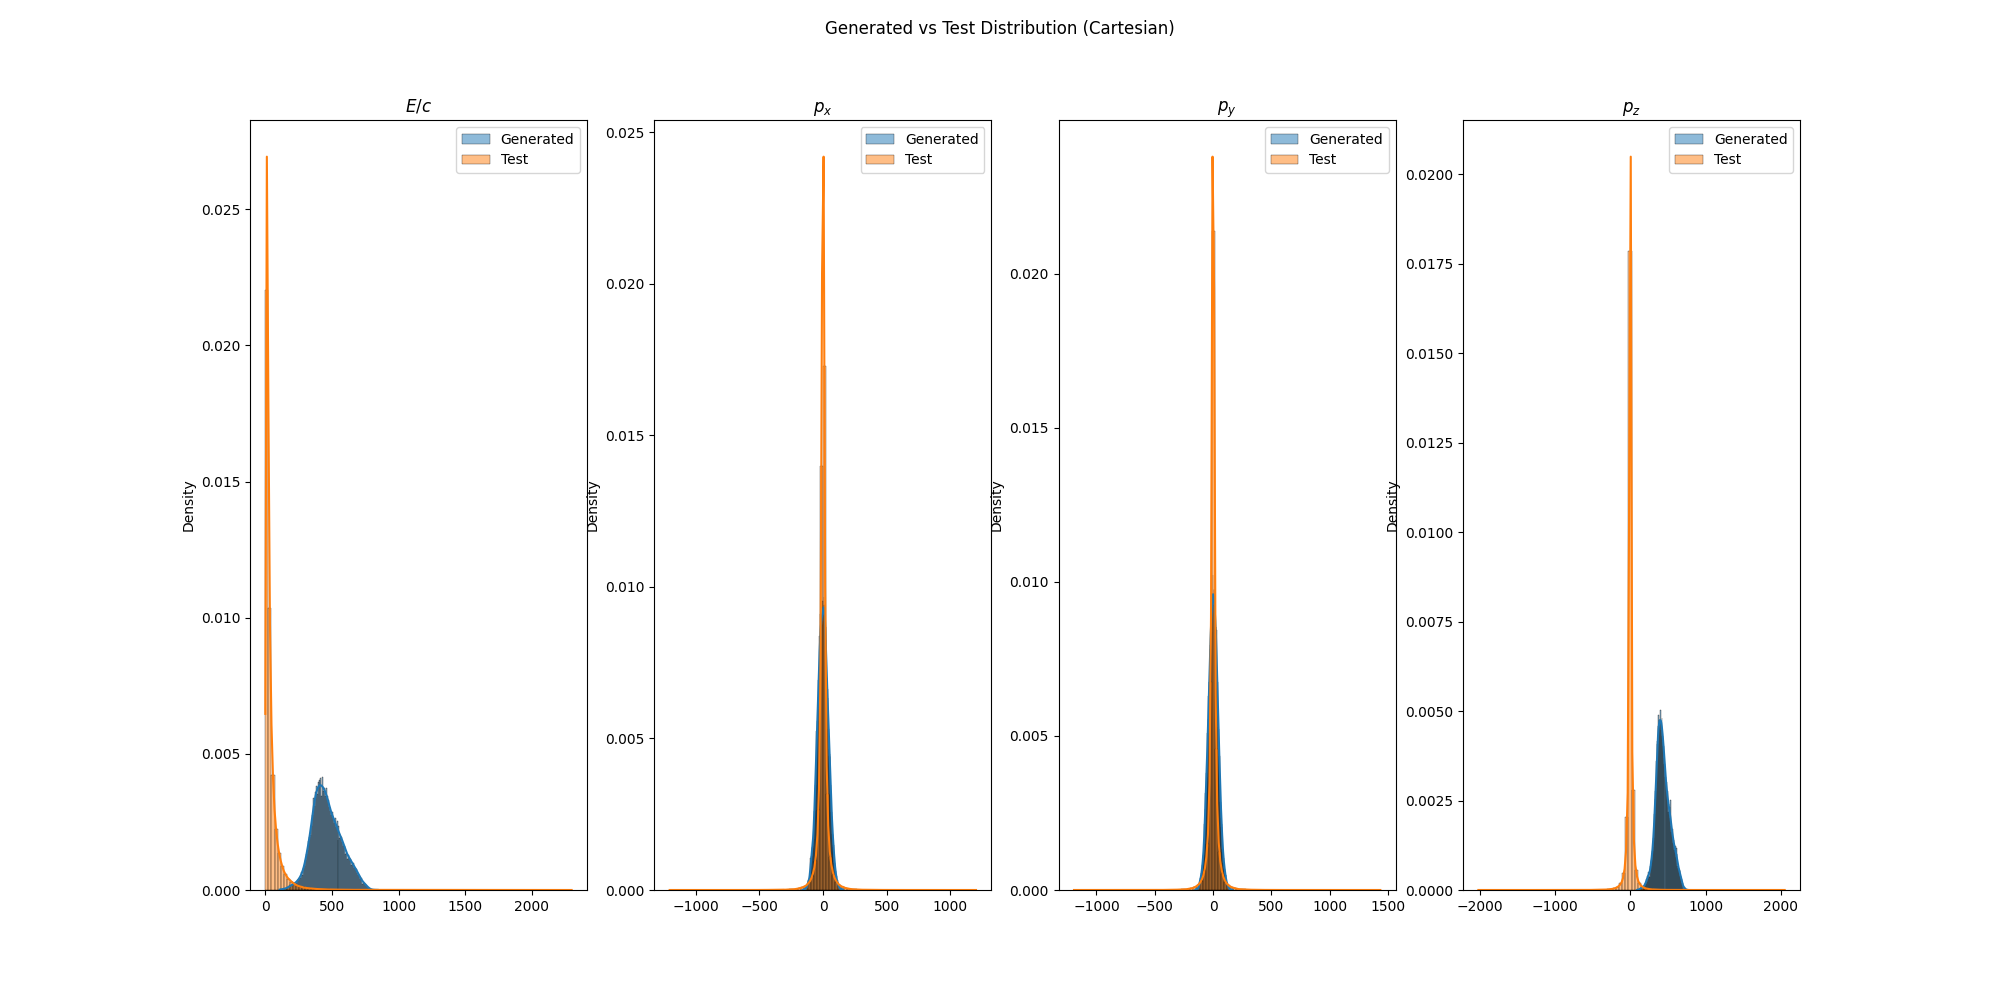
\includegraphics[width=0.8\textwidth]{figs/generated_vs_test_distribution_cartesian.png}
    \end{figure}
        \begin{figure}
        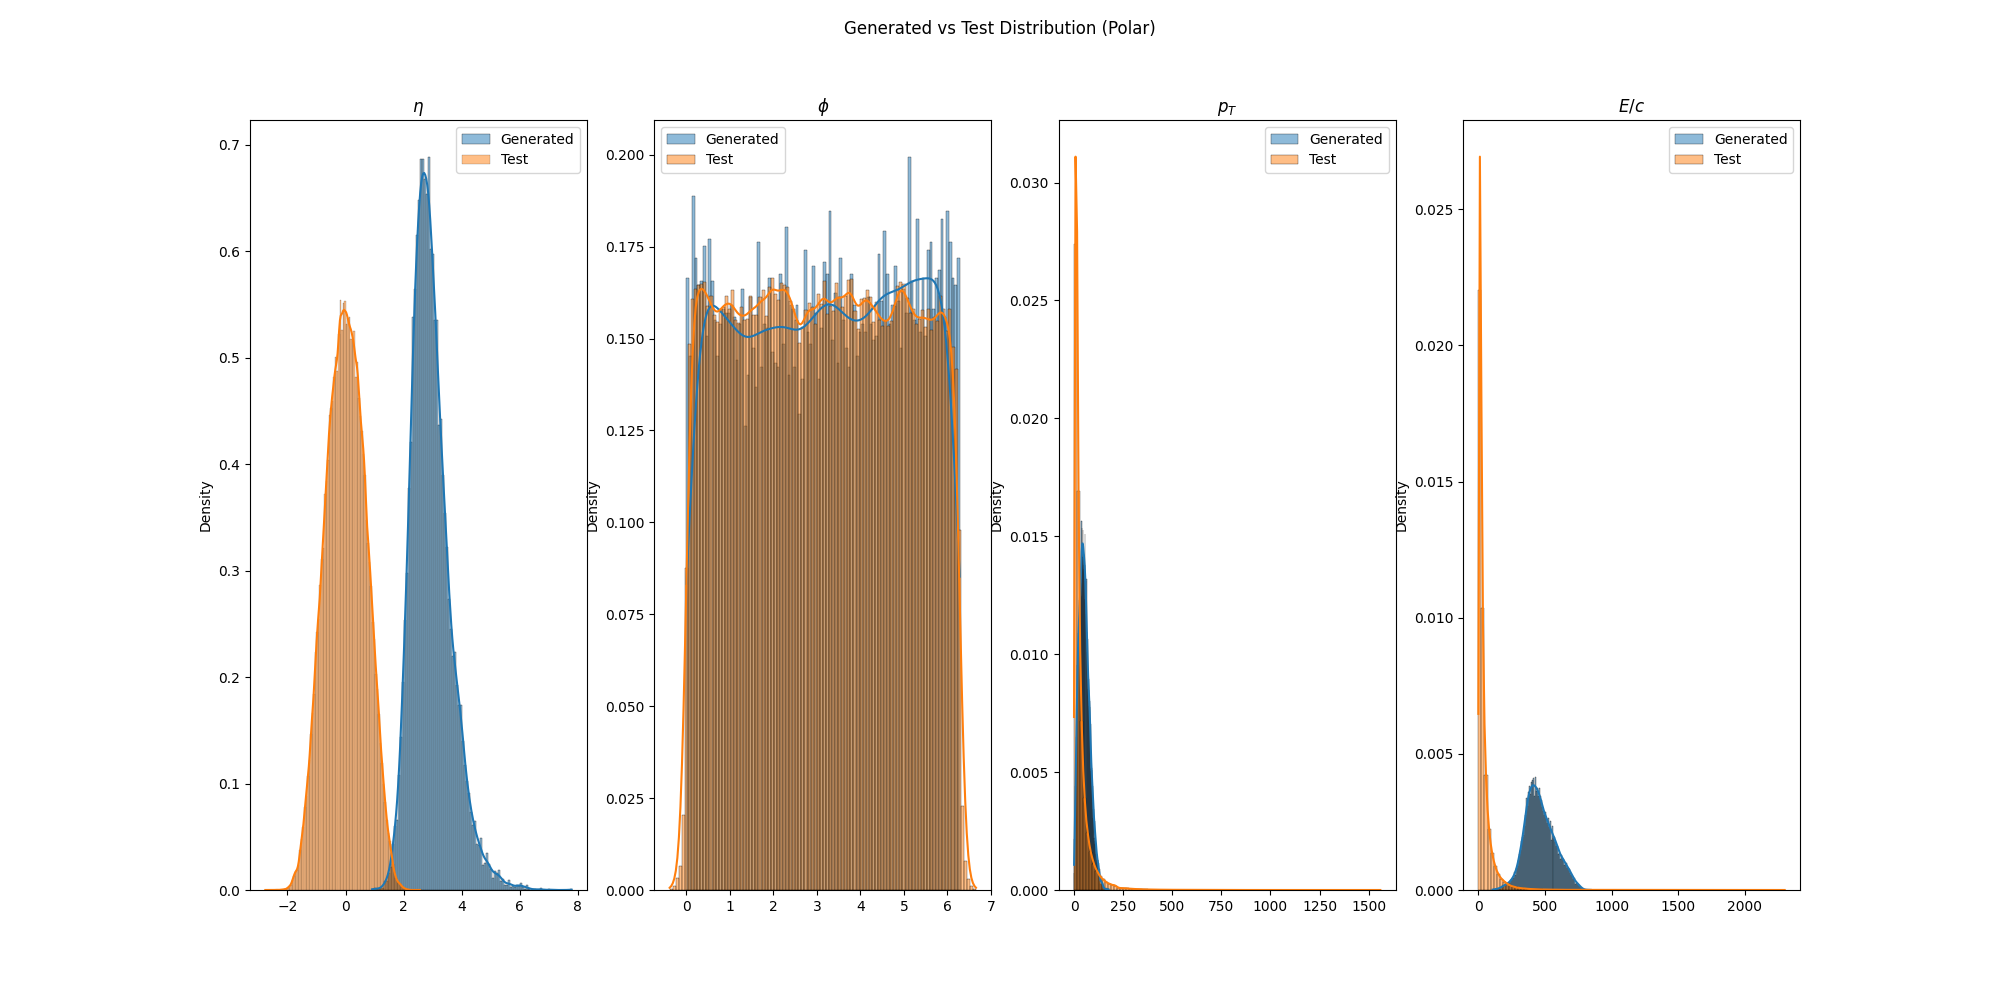
\includegraphics[width=0.8\textwidth]{figs/generated_vs_test_distribution_polar.png}
    \end{figure}

    \begin{table}
        \caption{Metrics relative to test set}
        \begin{tabular}{|c| c | c |}
            \hline
            Metric & Value & MPGAN Value \\ \hline
            Covariance ($\uparrow$) & 0.068 & 0.240 \\
            MMD ($\downarrow$) & 2.018 & 0.045 \\\hline
        \end{tabular}
    \end{table}
\end{frame}

\begin{frame}[allowframebreaks]{Inspiration for new architecture}
    \begin{figure}
        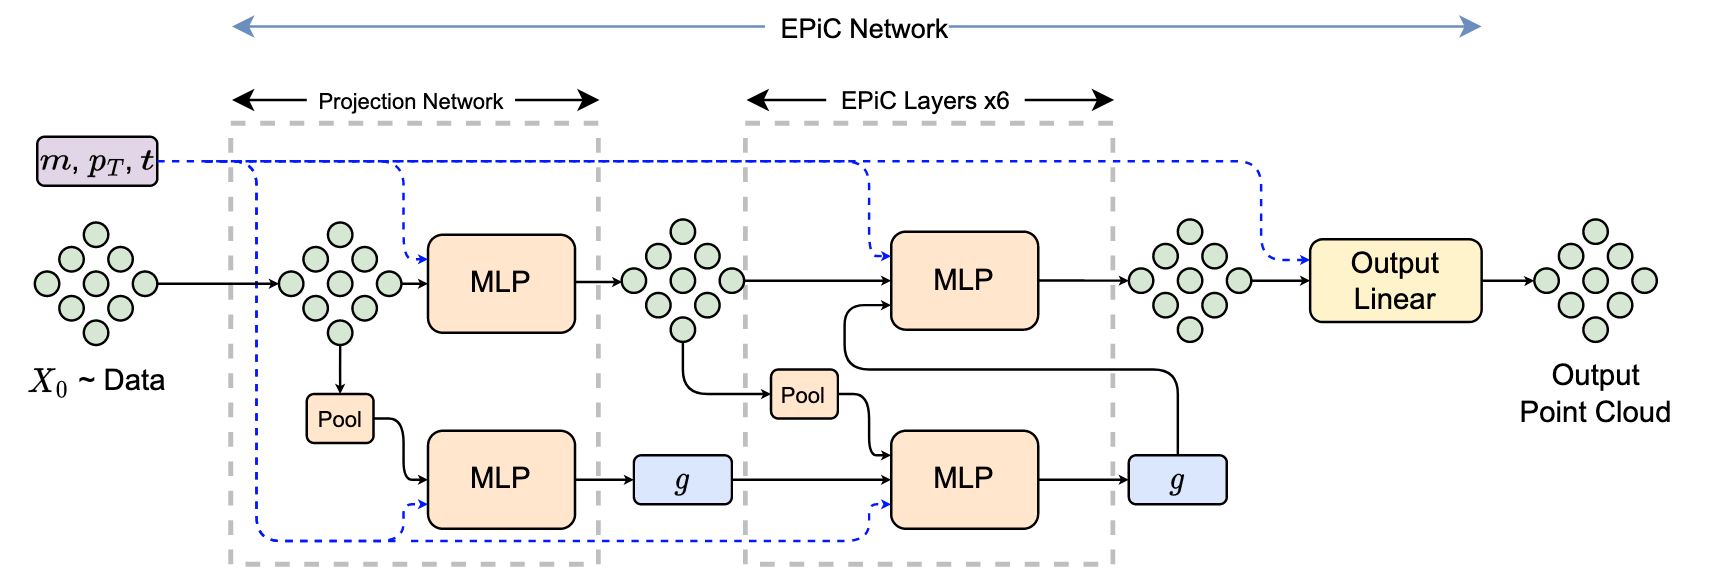
\includegraphics[height=0.6\textheight]{figs/epic-jedifm.png}
        \caption{EPiC-FM \cite{buhmannEPiClyFastParticle2023}}
    \end{figure}
    \begin{figure}
        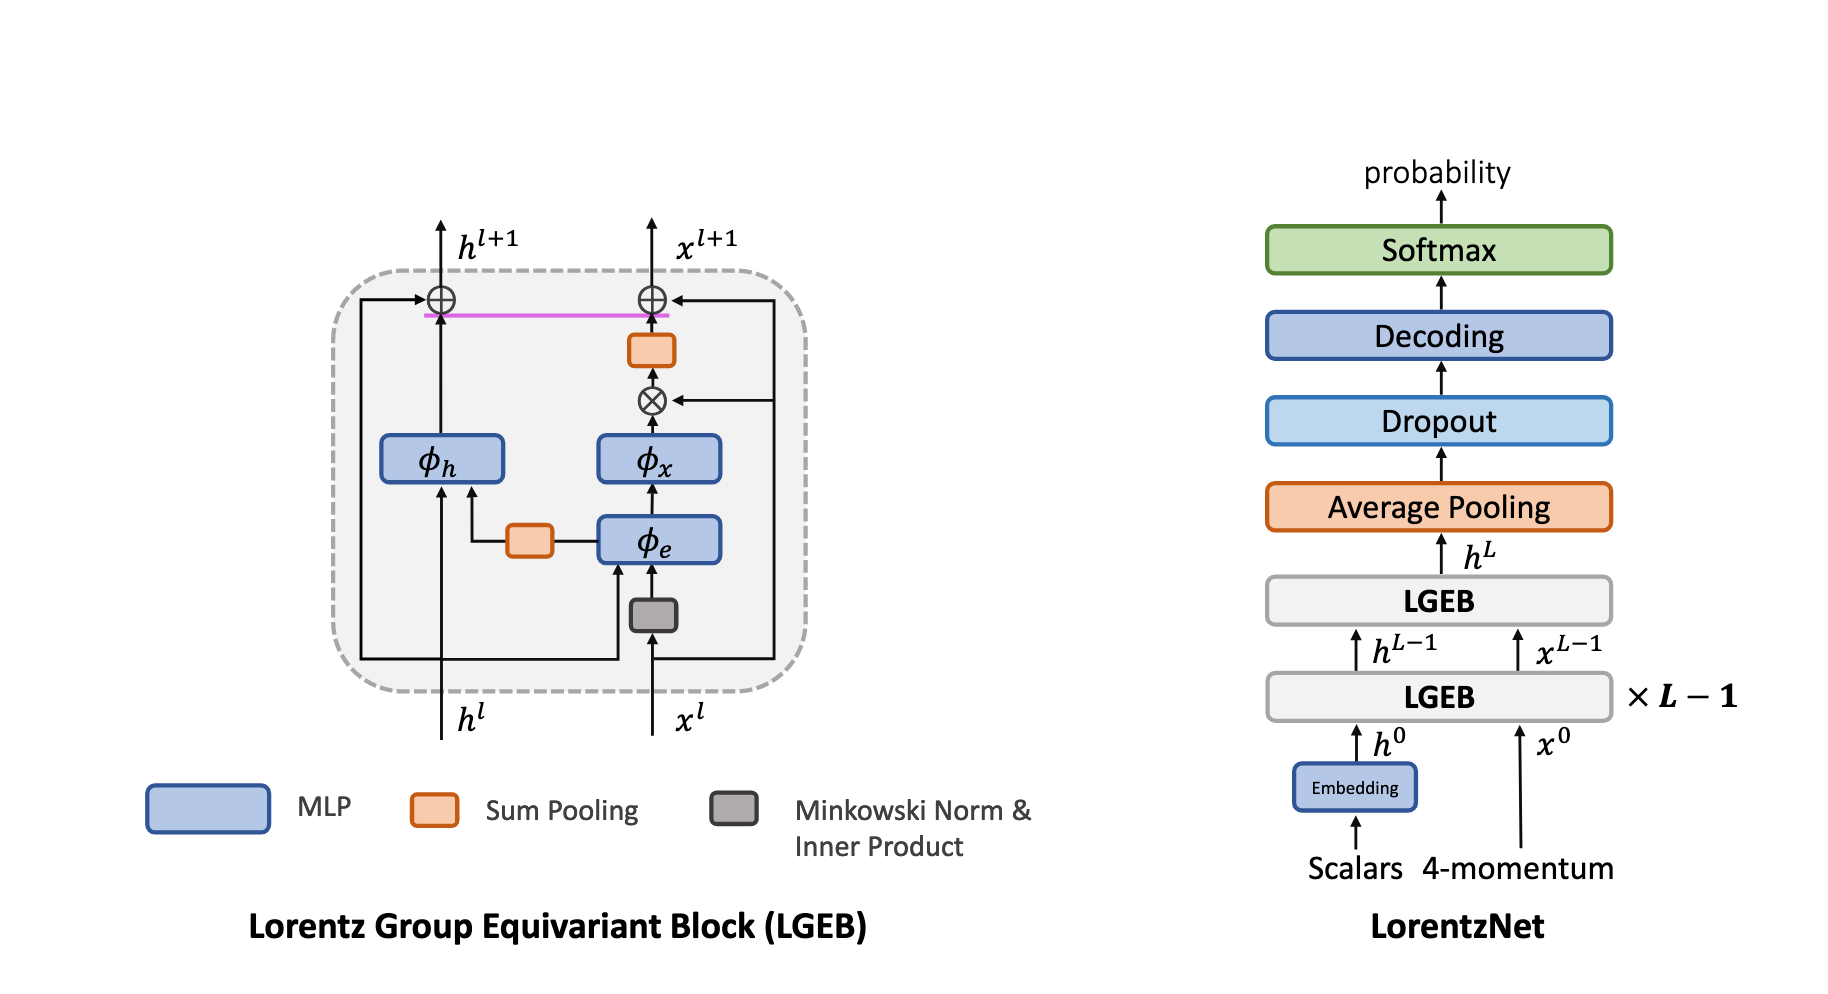
\includegraphics[height=0.75\textheight]{figs/lorentznet.png}
    \end{figure}
    \begin{figure}
        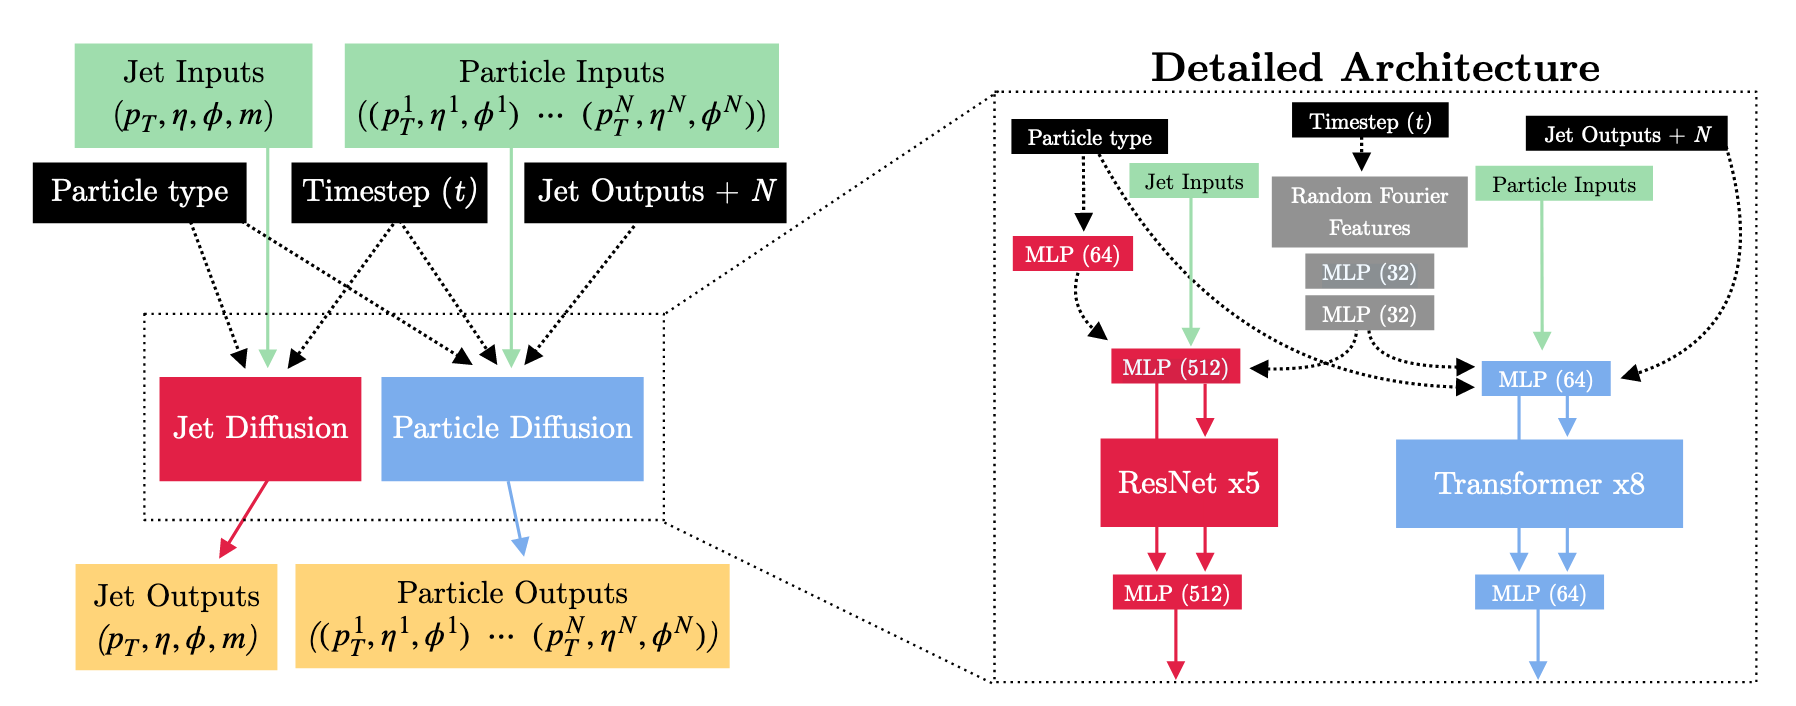
\includegraphics[width=0.6\textwidth]{figs/fpcd.png}
        \caption{FPCD \cite{wuFastPointCloud2023}}
    \end{figure}
\end{frame}

\begin{frame}{Implementation details for next training runs}
    \begin{itemize}
        \item AdamW \cite{loshchilovDecoupledWeightDecay2019} optimizer
        \item Learning rate: linear warm-up followed by cosine annealing (same as \cite{buhmannEPiClyFastParticle2023})
        \item LeakyRELU activation (negative slope = 0.01)
        \item Zero padding for variable-sized particle clouds
    \end{itemize}
\end{frame}

\begin{frame}{Zero padding}
    In each layer:
    \begin{itemize}
        \item Calculate edge features for all particles and multiply by expanded mask
        \item Multiply results of $\phi_e(m_{ij})$, $\phi_{x}(m_{ij})$ by expanded mask
        \item Keep track of valid edges for average pooling
        \item To guarantee the mask is respected, multiply node updates and final nodes by mask before passing to next layer
    \end{itemize}
\end{frame}

\begin{frame}{Learning rate}
    \begin{figure}
        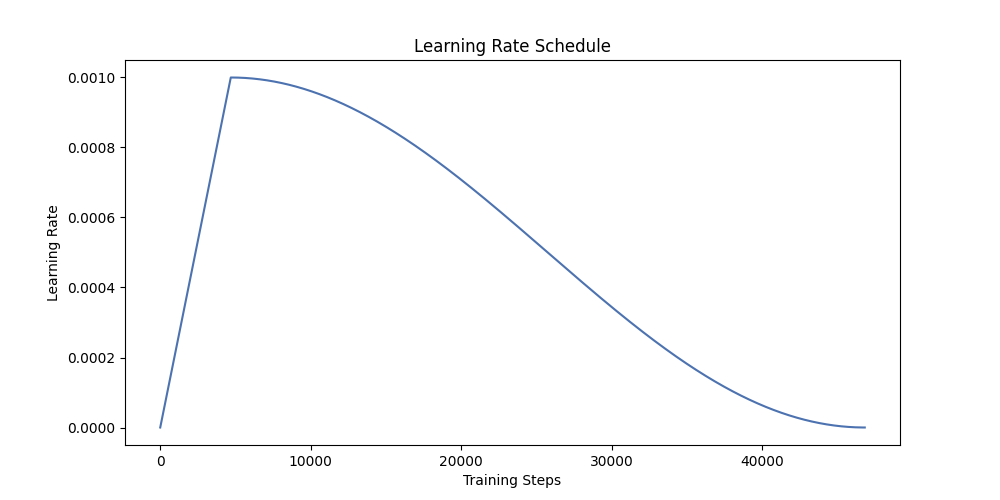
\includegraphics[width=0.8\textwidth]{figs/learning_rate_schedule.png}
        \caption{Linear warm-up followed by cosine annealing}
    \end{figure}
\end{frame}

\begin{frame}[allowframebreaks]{This week}
    \begin{itemize}
        \item Run jobs today: \begin{itemize}
            \item Entire dataset; $\approx$ 50 epochs; $\approx$ 8 layers
            \item Entire dataeset; $\approx$ 1000 epochs; $\approx$ 12 layers
        \end{itemize}
        \item Implement parallelized training with Hugging Face Accelerate
        \item Set up sampling pipeline while training the model to get an indication of how performance improves over time (since FM loss tends to be meaningless after the first epoch)
        \item Theoretical problems with equivariance \begin{itemize}
            \item Currently initializing from normal distribution
            \item Go over E(3)-equivariant papers in detail and try to develop something similar to CoM trick
        \end{itemize}
        \item Set up plots typically used in jet generation papers
        \item Mean flow setup (should be the first paper to use it for jets)
    \end{itemize}
\end{frame}


\begin{frame}[allowframebreaks]{References}
\printbibliography
\end{frame}
\end{document}
